%-------------------------------------------------------------------------------
% seq66 mutes
%-------------------------------------------------------------------------------
%
% \file        seq66 mutes.tex
% \library     Documents
% \author      Chris Ahlstrom
% \date        2020-01-13
% \update      2023-04-14
% \version     $Revision$
% \license     $XPC_GPL_LICENSE$
%
%     Provides a discussion of the MIDI GUI mutes that Seq66
%     supports.
%
%-------------------------------------------------------------------------------

\section{Seq66 Mutes Master}
\label{sec:mutes_master}

   The \textbf{Mutes} tab is a way to get a global view of all the mutegroups in
   a \textsl{Seq66} MIDI file or global configuration, and to be able to do
   some simple operations with the mute groups.
   A mute-group holds the statuses (armed/muted) of all of the patterns in
   a screenset (see \sectionref{subsubsec:concepts_terms_bank}).
   A mute-group can be associated with a hot-key (or MIDI control), so that,
   when the mute-group is selected, the patterns that are armed changes.
   This makes it easy to change what the tune is playing in a big way.
   Mute-groups are \textsl{learned} by

   \begin{enumerate}
      \item Arming all of the desired pattern in the set.
      \item Clicking the \textbf{Learn} ("L") button.
      \item Clicking the keystroke, which is almost always the shifted version
         of the hot-key to arm/mute the pattern.
         This is accomplished in the default keyboard configuration via the
         \index{auto-shift}
         auto-shift function, which shifts the keystroke automatically
         for group-learn.
   \end{enumerate}

   These steps can also be done via MIDI control.

   To learn more about mute-groups, see
   \sectionref{subsubsec:introduction_mute_group_learn_button}, and
   \sectionref{subsubsec:concepts_terms_group}.

% TODO: UPDATE THIS FIGURE WITH THE LATEST.

\begin{figure}[H]
   \centering 
   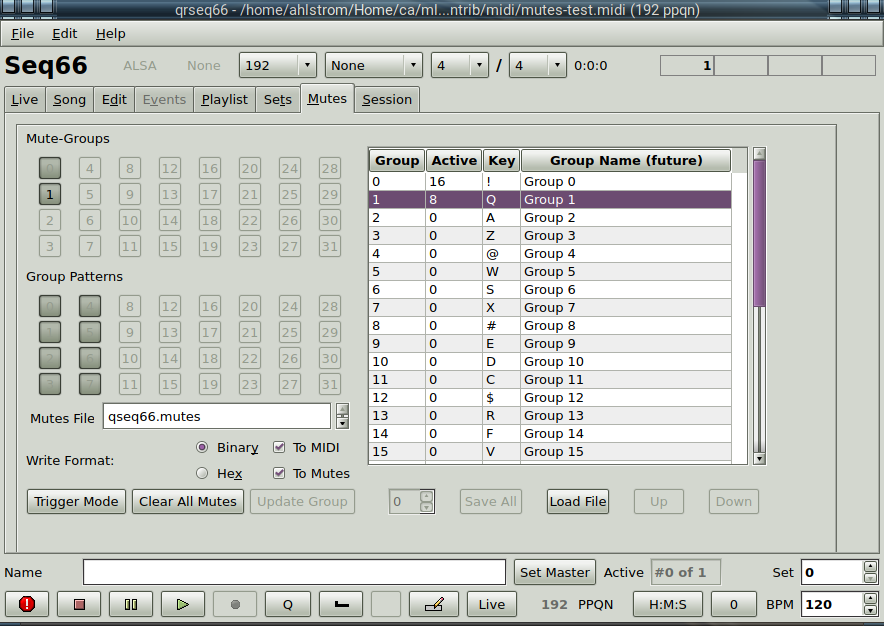
\includegraphics[scale=0.75]{tabs/mutes/mute-master-tab.png}
   \caption{Mutes Tab}
   \label{fig:mutes_master_tab}
\end{figure}

   This diagram show the \textbf{Mutes} tab after some mute-groups have been
   created.  Mute-groups can be created in the main window's patterns panel,
   but it is difficult to know what each group consists of.  This tab make it
   easy to see the layout of the mute-groups, and also allows for some editing
   of the mute-groups.

   \setcounter{ItemCounter}{0}      % Reset the ItemCounter for this list.

   \itempar{Group Table}{mutes!table}
   At the right is a table that holds all of the assigned mute-group key and
   some information about them:

      \begin{itemize}
         \item \textbf{Group}.
            This column holds the group numbers for each group, ranging from 0
            to 31.  Each row corresponds to a buton in the \textbf{Mute-Groups}
            grid.
         \item \textbf{Active}.
            This column shows the number of activated patterns in the
            mute-group.  A zero means the mute-group is inactive.
         \item \textbf{Key}.
            Indicates the keystroke that can be used to put that mute-group in
            place on the patterns in the current screenset.
            By default, these are shifted version of the corresponding
            mute/unmute pattern-slot hotkey.
         \item \textbf{Group Name}.
            Provides a mnemonic name for the mute group.  A feature for the
            future.
      \end{itemize}

   Currently, only the \textbf{Group Name} field is editable directly.
   The user generally should modify (tweak)
   \texttt{qseq66.mutes} with a text editor.
   This table is the only way to select a mute-group for editing.
   Click on the desired group, and then click on the group button, perhaps
   twice, to be able to add pattern mute states via the pattern buttons.

   \itempar{Mute-Groups}{mutes!groups}
   This grid is always of size \textbf{4 x 8}.  It represents the maximum of 32
   mute-groups that can be supported by \textsl{Seq66}.
   To start, all group buttons are \textsl{disabled} and
   \textsl{unchecked} (inactive).
   Where a mute-group exists, the button is made \textsl{checked} (active),
   but still disabled.

   Here, the user clicked on mute-group 7, which now becomes active in the
   user-interface.  (But it is not made active in the patterns panel).
   The \textbf{7} button is also enabled, and can be clicked.

   Clicking once deactivates the button, which potentially flags that mute-group
   for removal.  Clicking it again reactivates it, which also enables all of the
   buttons in the \textbf{Group Patterns} grid.

   \itempar{Group Patterns}{mutes!patterns}
   Once this grid is enabled, each button can be click to add a pattern to the
   mute-group, or remove a pattern from the mute-group.

   \itempar{Update Group}{mutes!update group}
%
%  Was "Set Mutes"
%
   When a change in the mute-group status or the status of one of its patterns
   is made, this button becomes enabled.  Once clicked, the current mute-group
   is modified internally, where it will later be saved when \textsl{Seq66}
   exits, or when the \textbf{Save All} button is clicked.

   \itempar{Mutes File}{mutes!mutes file}
   The mutes-file shows the base-name of a file into which one can write the
   current-mute group setup, as a way to back up the setup.
   TO DO:  We need to disable auto-save of the mutes file at exit in this case,
   unless the name provided is identical.

   \itempar{Save All}{mutes!save all}
%
%  Was "Save File"
%
   This button saves all of the mute-groups.
   It is enabled when a change has been made to a mute-group and
   has been registered by pressing the \textbf{Update Group} button.
   If the user has provided a path in the \textbf{Mutes File} field, the path
   is stripped.  We do not want to write configuration information outside of
   the session configuration directory.
   The file is saved, but is not made official in the
   'rc' file; one must edit the 'rc' file to use the new 'mutes' file.
   We might provide a button for that function at some point.

   \itempar{Write Format}{mutes!write format}
   This section provides the following features, which still need some work:

      \begin{itemize}
         \item \textbf{Binary}.
            This flag indicates to save the mute-group information in
            binary format, which is the normal format.
            Each mute-group pattern's setting is indicated by a 0 or a 1.
            This is the default format for writing the mute-groups.
         \item \textbf{Hex}.
            In this format, each set of mute-group is written in 8-bit hexadecimal
            format (e.g. "0xff").  This format is useful if the user has opted to
            have large set sizes such as 64 and 96 patterns.  Not well-supported
            yet.
         \item \textbf{To MIDI}.
            When a tune is closed, as when \textsl{Seq66} exits, this option
            indicates to write the mute-group information to the
            \textsl{Seq66}-style MIDI file.
         \item \textbf{To Mutes}.
            When a tune is closed, as when \textsl{Seq66} exits, this option
            indicates to write the mute-group information to the normal
            \textsl{Seq66} configuration file (e.g. \texttt{qseq66.mutes}).
      \end{itemize}

   \itempar{Trigger Mode}{mutes!trigger mode}
      When activated, this option will enable the \textbf{Mute-Groups} buttons,
      deactive them all, and turn them into standard push-buttons.  When clicked
      the mute-group will be actived during playback.

   \itempar{Clear}{mutes!clear all mutes}
      This button will clear every mute group. Use it carefully!

   \itempar{Fill}{mutes!fill mutes}
      This button will create a set of empty mute-groups.
      Currently, this alters the current MIDI tune, forcing a prompt to save.
      This action creates 32 empty mute-groups.
      If a single mute-group is created in the patterns panel,
      then only that mute-groups is saved.

% INVESTIGATE!!!

   \itempar{Pattern Offset}{mutes!pattern offset}
      If the user has selected a larger set size that is a multiple of 32, this
      item is enabled.  It then allows the user to modify patterns with a
      sequence number greater than 31.  A future feature.

   \itempar{Up/Down Buttons}{mutes!up/down buttons}
      A future feature to move mute-group around without
      changing the keystroke for that mute group.

%-------------------------------------------------------------------------------
% vim: ts=3 sw=3 et ft=tex
%-------------------------------------------------------------------------------
